\documentclass{article}

% NeurIPS 2024 format (preprint for arXiv)
\usepackage[preprint]{neurips_2024}

\usepackage[utf8]{inputenc}
\usepackage[T1]{fontenc}
\usepackage{hyperref}
\usepackage{url}
\usepackage[numbers,sort&compress]{natbib}
\usepackage{booktabs}
\usepackage{amsfonts}
\usepackage{amsmath}
\usepackage{nicefrac}
\usepackage{microtype}
\usepackage{xcolor}
\usepackage{graphicx}
\usepackage{subcaption}
\usepackage{multirow}
\usepackage{enumitem}

% Prevent ugly word spacing from dense citation blocks
\emergencystretch=1em

\title{Democratizing Agentic AI: Quantifying Reasoning Stability of Quantized SLMs in Recursive Agentic Loops on Resource-Constrained Hardware}

\author{%
  Farhan Zarif \\
  BRAC University \\
  Dhaka, Bangladesh \\
  \texttt{farhan.zarif1@g.bracu.ac.bd} \\
}

\begin{document}

\maketitle

\begin{abstract}
We present the first systematic evaluation of multi-turn recursive stability in quantized Small Language Models (SLMs) operating as autonomous agents on resource-constrained hardware. We test four SLMs---Gemma-3-4B, Llama-3.1-8B, Phi-4-Mini, and Qwen-3.5-4B---under 4-bit NF4 and 8-bit INT8 quantization on a 15\,GB VRAM Google Colab T4 GPU. Across 476 agentic tasks spanning Bash administration, Python debugging, and multi-hop Web synthesis, we introduce two novel evaluation metrics: the \textbf{Stability Decay Metric (SDM)}, which penalizes multi-turn inefficiency, and the \textbf{Quantization-Hallucination Ratio (QHR)}, which isolates structural formatting failures from logical reasoning errors. Our results reveal that (i)~Gemma-3-4B achieves the highest agentic stability ($\overline{\text{SDM}}=0.403$, success rate $53.3\%$ [95\% CI: 43.8, 62.6]), while Llama-3.1-8B fails catastrophically ($0.86\%$ [0.02, 4.71] success) due to persistent single-step repetition loops; (ii)~the effect of quantization precision is \emph{environment-dependent}: 4-bit significantly outperforms 8-bit in Bash ($p=0.044$), while 8-bit significantly outperforms 4-bit in Python ($p=0.009$); and (iii)~format/parser errors, not logical reasoning failures, constitute the dominant failure mode ($42.7\%$). Through qualitative analysis of 476 reasoning traces, we identify four distinct failure archetypes---\emph{reasoning leakage}, \emph{single-step stagnation}, \emph{code truncation}, and \emph{verification omission}---providing actionable deployment guidelines for quantized SLM agents on edge hardware. Code and data: \texttt{[redacted for review]}.
\end{abstract}

% ============================================================
\section{Introduction}
% ============================================================

By early 2026, a range of highly capable Small Language Models (SLMs) with sub-10B parameters have become available, including Alibaba's Qwen~3.5~\cite{bai2023qwen}, Google's Gemma~3~\cite{gemma2025}, Meta's Llama~3.1~\cite{touvron2023llama}, and Microsoft's Phi-4-Mini~\cite{phi4mini2025}. These models achieve competitive reasoning performance on static benchmarks while fitting within the memory constraints of consumer-grade GPUs~\cite{zhang2024tinyllama}, enabling a paradigm shift toward locally deployed, privacy-preserving AI agents~\cite{wang2024survey}.

However, deploying SLMs as \emph{autonomous agents}---where the model must maintain coherent reasoning across multiple recursive turns of planning, execution, observation, and self-correction~\cite{yao2022react}---introduces compounding failure modes that static benchmarks fail to capture~\cite{dong2025acbench,liu2023agentbench}. When these agents run on resource-constrained hardware (e.g., Google Colab's free-tier NVIDIA T4 GPU with $\sim$15\,GB VRAM), aggressive quantization via \texttt{bitsandbytes}~\cite{dettmers2022llm,dettmers2023qlora} is often required, yet its effects on multi-turn agentic stability remain poorly understood~\cite{colm2025quantization}.

\paragraph{Contributions.} This paper makes three contributions:
\begin{enumerate}[nosep]
  \item We introduce the \textbf{Stability Decay Metric (SDM)} and \textbf{Quantization-Hallucination Ratio (QHR)} to disentangle agentic efficiency from structural formatting integrity.
  \item We conduct the first systematic evaluation of \textbf{multi-turn recursive stability} in quantized SLM agents across \textbf{4 models $\times$ 2 precisions $\times$ 3 environments $\times$ 20 tasks = 480 experimental configurations} (476 completed), identifying statistically significant, environment-dependent quantization effects.
  \item Through qualitative trace analysis, we identify \textbf{four failure archetypes} specific to quantized agentic SLMs, providing actionable deployment guidelines.
  \item We propose \textbf{Agentic Sub-Capability Decomposition (ASCD)}, a framework decomposing multi-step agentic reasoning into four independently degradable sub-capabilities---plan decomposition, state tracking, format adherence, and completion signaling---enabling targeted diagnosis and mitigation.
\end{enumerate}

% ============================================================
\section{Related Work}
% ============================================================

\paragraph{Post-Training Quantization.}
Post-training quantization is the primary technique for deploying LLMs on consumer hardware. LLM.int8()~\cite{dettmers2022llm} showed that 8-bit matrix multiplication preserves transformer quality; QLoRA~\cite{dettmers2023qlora} introduced NF4 with double quantization. Subsequent methods include GPTQ~\cite{frantar2023gptq} (one-shot weight quantization), AWQ~\cite{lin2024awq} (activation-aware scaling), SqueezeLLM~\cite{kim2024squeezellm} (dense-and-sparse), OmniQuant~\cite{shao2024omniquant} (omnidirectional calibration), and AQLM~\cite{egiazarian2024aqlm} (additive codebooks). The 1-bit regime~\cite{ma2024era} remains impractical for agents; knowledge distillation~\cite{xu2024chatglm} is orthogonal. We use bitsandbytes NF4 and INT8 as the most widely deployed open-source methods.

\paragraph{Agent Frameworks and Benchmarks.}
ReAct~\cite{yao2022react} established thought-action-observation loops; Toolformer~\cite{schick2023toolformer} taught models API use via self-supervision; Reflexion~\cite{shinn2023reflexion} introduced verbal reinforcement learning related to our Actor-Critic loop; SWE-agent~\cite{yang2024sweagent} applied agentic loops to software engineering; AutoGPT~\cite{autogpt2023} and MetaGPT~\cite{hong2024metagpt} demonstrated end-to-end autonomous agent systems with multi-step planning. Surveys~\cite{wang2024survey,xi2023rise} establish that effective agency requires compositional capabilities (planning, tool use, memory, self-correction), building on chain-of-thought reasoning~\cite{wei2022chainofthought}. Among benchmarks, AgentBench~\cite{liu2023agentbench} tests across 8 environments, WebArena~\cite{zhou2024webarena} and OSWorld~\cite{xie2024osworld} target realistic settings, T-Eval~\cite{chen2024teval} evaluates step-by-step tool use, and ToolLLM~\cite{qin2024toolllm} scales to 16K+ APIs. ACBench~\cite{dong2025acbench} (ICML 2025) most directly evaluates \emph{compressed} agents across workflows, tool use, and long-context tasks, but focuses on compression-method comparison (pruning vs.\ quantization) for large LLMs (7B--70B) rather than \emph{recursive stability decay}: it does not measure turn-level efficiency degradation, self-correction dynamics, or failure-archetype taxonomy in quantized SLMs on resource-constrained hardware. Our work fills this gap.

\paragraph{Quantization and Reasoning.}
COLM 2025~\cite{colm2025quantization} shows quantization disproportionately impacts reasoning, but focuses on static benchmarks. Huang and Chang~\cite{huang2023reasoning} establish reasoning as a multi-component capability; SLM surveys~\cite{slm2025survey} identify the need for deployment recommendations. TinyLLM~\cite{tinyllm2025} evaluates fine-tuning strategies for sub-3B SLMs on function-calling tasks; we evaluate quantization effects on larger SLMs (3.8--8B) across multi-turn recursive execution. However, no prior work examines how quantization affects \emph{recursive stability decay}---the compounding degradation of agentic sub-capabilities across turns $t \rightarrow t{+}k$---with turn-level efficiency metrics and failure-archetype diagnosis.

% ============================================================
\section{Methodology}
% ============================================================

\subsection{Experimental Design and Task Prompts}

We evaluate four SLMs under two quantization levels across three agentic environments, yielding a $4 \times 2 \times 3 = 24$ configuration grid. Each configuration is tested on 20 tasks, producing 480 planned trials (476 completed; 4 Llama-3.1 tasks terminated due to VRAM pressure). Experiments were conducted March 3--12, 2026, on Google Colab free-tier NVIDIA T4 GPUs ($\sim$15\,GB VRAM).

The 60 prompts (20/env) are imperative, self-contained instructions with deterministically verifiable outputs. \textbf{Bash} covers directory manipulation, text pipelines (\texttt{grep}/\texttt{sed}), permissions, and archival (1--5 step pipelines). \textbf{Python} spans DSA (BST, Sieve, Levenshtein), OOP, concurrency, and I/O (10--50 lines). \textbf{Web} requires multi-hop research over a 40-entry knowledge base ($\geq$2 searches + synthesis). Complexity: $\sim$30\% single-step, $\sim$50\% 2--3 steps, $\sim$20\% 4--5 interdependent steps.

\subsection{Inference Pipeline}

Models load via \texttt{bitsandbytes}~\cite{dettmers2022llm}: NF4 4-bit with double quantization and \texttt{float16} compute; INT8 via \texttt{load\_in\_8bit}. Hyperparameters: $T{=}0.7$~\cite{wang2024survey}, $p{=}0.9$, max\_tokens${=}400$.

\subsection{Agentic Loop}

We implement a ReAct-style~\cite{yao2022react} recursive loop ($D_{\max}{=}5$ turns): the agent receives the objective and compressed trajectory, produces a \texttt{<thought>} trace, emits an action, and observes the result. \textbf{Sliding-window trajectory injection} compresses the execution history into a structured Turn/Action/Outcome representation, retains only the most recent 2 turn-pairs (whitespace-normalized, outcomes truncated to 500 chars), and injects this context into the next prompt to prevent context saturation. \textbf{Actor-Critic Self-Correction}: before execution, the same SLM re-evaluates the action (``Identify flaws. If perfect, output SAFE''); corrections replace originals.

\textbf{Environments.} \textbf{Bash} (Env~A): one command in \texttt{```bash} blocks, 10s timeout---tests structural adherence. \textbf{Python} (Env~B): complete scripts in \texttt{```python} blocks, 15s timeout with traceback feedback---tests iterative debugging. \textbf{Web} (Env~C): JSON \texttt{search}/\texttt{answer} actions over a 40-entry knowledge base---tests cross-turn coherence.

\subsection{Models}

Table~\ref{tab:models} summarizes the four SLMs evaluated. All configurations fit within the 15\,GB T4 VRAM constraint, with 4-bit achieving $1.5$--$2\times$ VRAM reduction.

\begin{table}[ht]
\caption{Model roster with measured VRAM allocations under each quantization level.}
\label{tab:models}
\centering
\small
\begin{tabular}{@{}llcc@{}}
\toprule
Model & Params & 4-bit VRAM & 8-bit VRAM \\
\midrule
\texttt{gemma-3-4b-it}~\cite{gemma2025} & 4B & 3.03--6.16\,GB & 4.68\,GB \\
\texttt{Llama-3.1-8B-Instruct}~\cite{touvron2023llama} & 8B & 5.32\,GB & 8.47\,GB \\
\texttt{Phi-4-mini-instruct}~\cite{phi4mini2025} & 3.8B & 2.70\,GB & 4.16\,GB \\
\texttt{Qwen3.5-4B}~\cite{bai2023qwen} & 4B & 2.91\,GB & 4.54\,GB \\
\bottomrule
\end{tabular}
\end{table}

\subsection{Evaluation Metrics}

\paragraph{Stability Decay Metric (SDM).} Agentic efficiency degrades with increasing turn count:
\begin{equation}
  \text{SDM} = \mathbb{I}_{\text{success}} \times \left(1 - \frac{T - 1}{D_{\max}}\right)
\end{equation}
where $\mathbb{I}_{\text{success}} = 1$ if the task is solved (validated by LLM-as-a-Judge), $T$ is turns used, $D_{\max} = 5$.

\paragraph{QHR.} Format violations break the parsing loop. QHR $= \sum_{t=1}^{T} \mathbb{I}_{\text{parser\_error}}(t) / T$.

\paragraph{Supplementary Metrics.} (i)~\textbf{Thinking Integrity}: binary tag-structure adherence; (ii)~\textbf{Reasoning Trace Length}: character count within \texttt{<thought>} tags; (iii)~\textbf{Self-Corrections}: Actor-Critic modifications; (iv)~\textbf{Backtracking}: consecutive error-state turns.

\subsection{Qualitative Coding Protocol}
\label{sec:coding}

Failure archetypes were derived via inductive thematic coding of all 24 Output.md trace logs. \textbf{Open coding} assigned descriptive labels (``tag leakage,'' ``repeated command,'' ``truncated output'') to each failure. \textbf{Axial coding} grouped codes by causal mechanism (structural vs.\ logical). \textbf{Selective coding} yielded four saturated archetypes: Reasoning Leakage ($n{=}58$), Single-Step Stagnation ($n{=}62$), Code Truncation ($n{=}27$), Verification Omission ($n{=}18$). Saturation confirmed after 18/24 files. To mitigate single-coder bias, we developed an automated regex-based archetype detector that independently classified all 398 parseable tasks; the automated tool recovered the same dominant archetype per model (Qwen$\to$Leakage, Llama$\to$Stagnation, Gemma$\to$Truncation, Phi$\to$Omission), providing triangulation of the manual coding. Single-coder limitation acknowledged in Section~\ref{sec:limitations}.

\subsection{Validation}

Task completion uses an LLM-as-a-Judge (same quantized model): receives task objective + final state (1000 chars), emits \texttt{[VERDICT: YES/NO]}. Manual review of 50 rejected tasks estimates $\sim$12\% false-negative rate (6/50), primarily Phi-4-Mini (Section~\ref{sec:limitations}).

% ============================================================
\section{Results}
% ============================================================

\subsection{Overall Performance}

Table~\ref{tab:results} presents comprehensive results across all 24 configurations. The overall success rate was 29.6\% (141/476).

\begin{table}[h]
\caption{Performance across all 24 configurations. Bold = best per-environment.}
\label{tab:results}
\centering
\scriptsize
\begin{tabular}{@{}llccccccc@{}}
\toprule
Model & Prec. & Env & Succ.\% & SDM & QHR & Turns & Lat. (s) & VRAM \\
\midrule
\multirow{6}{*}{Gemma-3}
 & 4-bit & Bash & 35.0 & .240$\pm$.162 & .037 & 2.4 & 40.9 & 6.09 \\
 & 4-bit & Py & 35.0 & .270$\pm$.190 & .075 & 4.0 & 243.0 & 3.03 \\
 & 4-bit & Web & \textbf{85.0} & \textbf{.640}$\pm$.134 & .020 & 2.4 & 45.9 & 6.16 \\
 & 8-bit & Bash & 10.0 & .040$\pm$.065 & .160 & 4.6 & 187.5 & 4.68 \\
 & 8-bit & Py & \textbf{70.0} & \textbf{.660}$\pm$.213 & .102 & 1.5 & 162.0 & 4.68 \\
 & 8-bit & Web & \textbf{85.0} & .570$\pm$.126 & .017 & 2.6 & 63.5 & 4.68 \\
\midrule
\multirow{6}{*}{Llama-3.1}
 & 4-bit & Bash & 0.0 & .000 & .244 & 5.0 & 116.9 & 5.32 \\
 & 4-bit & Py & 0.0 & .000 & .116 & 5.0 & 265.6 & 5.32 \\
 & 4-bit & Web & 0.0 & .000 & .080 & 5.0 & 68.9 & 5.32 \\
 & 8-bit & Bash & 0.0 & .000 & .250 & 4.7 & 186.4 & 8.47 \\
 & 8-bit & Py & 5.3 & .032$\pm$.066 & .053 & 4.9 & 483.3 & 8.47 \\
 & 8-bit & Web & 0.0 & .000 & .000 & 4.8 & 74.4 & 8.47 \\
\midrule
\multirow{6}{*}{Phi-4-Mini}
 & 4-bit & Bash & 5.0 & .040$\pm$.084 & .325 & 2.8 & 46.5 & 2.70 \\
 & 4-bit & Py & 35.0 & .290$\pm$.205 & .070 & 2.4 & 46.1 & 2.70 \\
 & 4-bit & Web & 45.0 & .320$\pm$.176 & .000 & 3.5 & 25.2 & 2.70 \\
 & 8-bit & Bash & 5.0 & .030$\pm$.063 & .143 & 3.4 & 84.4 & 4.16 \\
 & 8-bit & Py & 40.0 & .380$\pm$.227 & .200 & 1.4 & 59.1 & 4.16 \\
 & 8-bit & Web & 50.0 & .250$\pm$.128 & .000 & 3.9 & 41.2 & 4.16 \\
\midrule
\multirow{6}{*}{Qwen-3.5}
 & 4-bit & Bash & 15.0 & .110$\pm$.127 & .428 & 3.7 & 360.5 & 2.91 \\
 & 4-bit & Py & 10.0 & .080$\pm$.115 & .252 & 3.9 & 350.1 & 2.91 \\
 & 4-bit & Web & 40.0 & .230$\pm$.147 & .308 & 3.6 & 217.2 & 2.91 \\
 & 8-bit & Bash & 45.0 & .170$\pm$.102 & .430 & 3.9 & 759.6 & 4.54 \\
 & 8-bit & Py & 35.0 & .240$\pm$.171 & .190 & 3.1 & 633.0 & 4.54 \\
 & 8-bit & Web & 55.0 & .310$\pm$.153 & .354 & 3.9 & 475.5 & 4.54 \\
\bottomrule
\end{tabular}
\end{table}

Gemma-3 dominates ($\overline{\text{SDM}}=0.403$, 53.3\% success [95\% binomial CI: 43.8, 62.6]). Phi-4-Mini (30.0\% [21.6, 39.5]) and Qwen-3.5 (33.3\% [24.6, 43.1]) perform comparably, while Llama-3.1 exhibits near-total failure (0.86\% [0.02, 4.71], 1/116 tasks), despite being the largest model at 8B. The non-overlapping CIs between Gemma-3 and Llama-3.1 confirm that their performance difference is robust to sampling variability.

\subsection{4-bit vs.\ 8-bit: Environment-Dependent Effects}

Mann-Whitney $U$ tests ($n=20$ per group) reveal that quantization effects are \emph{not uniform}. In Bash, 4-bit Gemma-3 \emph{significantly outperforms} 8-bit ($\Delta\text{SDM}=+0.200$, $U=255$, $p=0.044$, rank-biserial $r=0.275$). In Python, 8-bit \emph{significantly outperforms} 4-bit ($\Delta\text{SDM}=+0.390$, $U=110.5$, $p=0.009$, $r=0.448$, a medium-to-large effect). Qwen-3.5 shows a trending Python advantage for 8-bit ($p=0.078$, $r=0.255$). All other 9 comparisons are non-significant ($p>0.10$).

\subsection{Qualitative Failure Archetypes}
\label{sec:qualitative}

Through systematic qualitative coding of 476 traces (Section~\ref{sec:coding}), we identify four archetypes:

\paragraph{A1: Reasoning Leakage (Qwen-3.5, $n{=}58$).}
Qwen-3.5 uses native \texttt{</think>} tags instead of prompted \texttt{<thought>} tags, creating dual-tag confusion. Under quantization, reasoning text leaks into executable blocks, producing errors like \texttt{/bin/sh: 1: The: not found}. QHR: $\overline{0.327}$, highest of all models (Fig.~\ref{fig:selfcorr_qhr}c--d).

\paragraph{A2: Single-Step Stagnation (Llama-3.1, $n{=}62$).}
Llama-3.1 correctly identifies the first step but repeats it across all turns (e.g., \texttt{mkdir -p project/src} on all 5 turns). Self-corrections trigger $\overline{3.2}\times$/task but cannot alter the trajectory---a fundamental state-tracking failure producing a stateless agent.

\paragraph{A3: Code Truncation (Gemma-3 Python, $n{=}27$).}
Correct reasoning traces yield truncated code. On the Levenshtein task (py\_8), Gemma-3 8-bit correctly described the DP approach across 5 turns but truncated at \texttt{if s1[i - 1} three times (SyntaxError). The 8-bit variant has significantly fewer truncations ($p=0.009$), linking truncation to 4-bit's degraded long-range syntactic attention. The Actor-Critic provides within-turn repair but cannot prevent cross-turn recurrence.

\paragraph{A4: Verification Omission (Phi-4-Mini, $n{=}18$).}
Phi-4-Mini executes correct commands but omits \texttt{[TASK\_COMPLETE]} or provides insufficient evidence for the judge. This inflates failure rates: $\sim$12\% of Phi-4-Mini rejections are false negatives.

\subsection{Self-Correction, Reasoning Traces, and Stability Decay}

\begin{figure}[t]
  \centering
  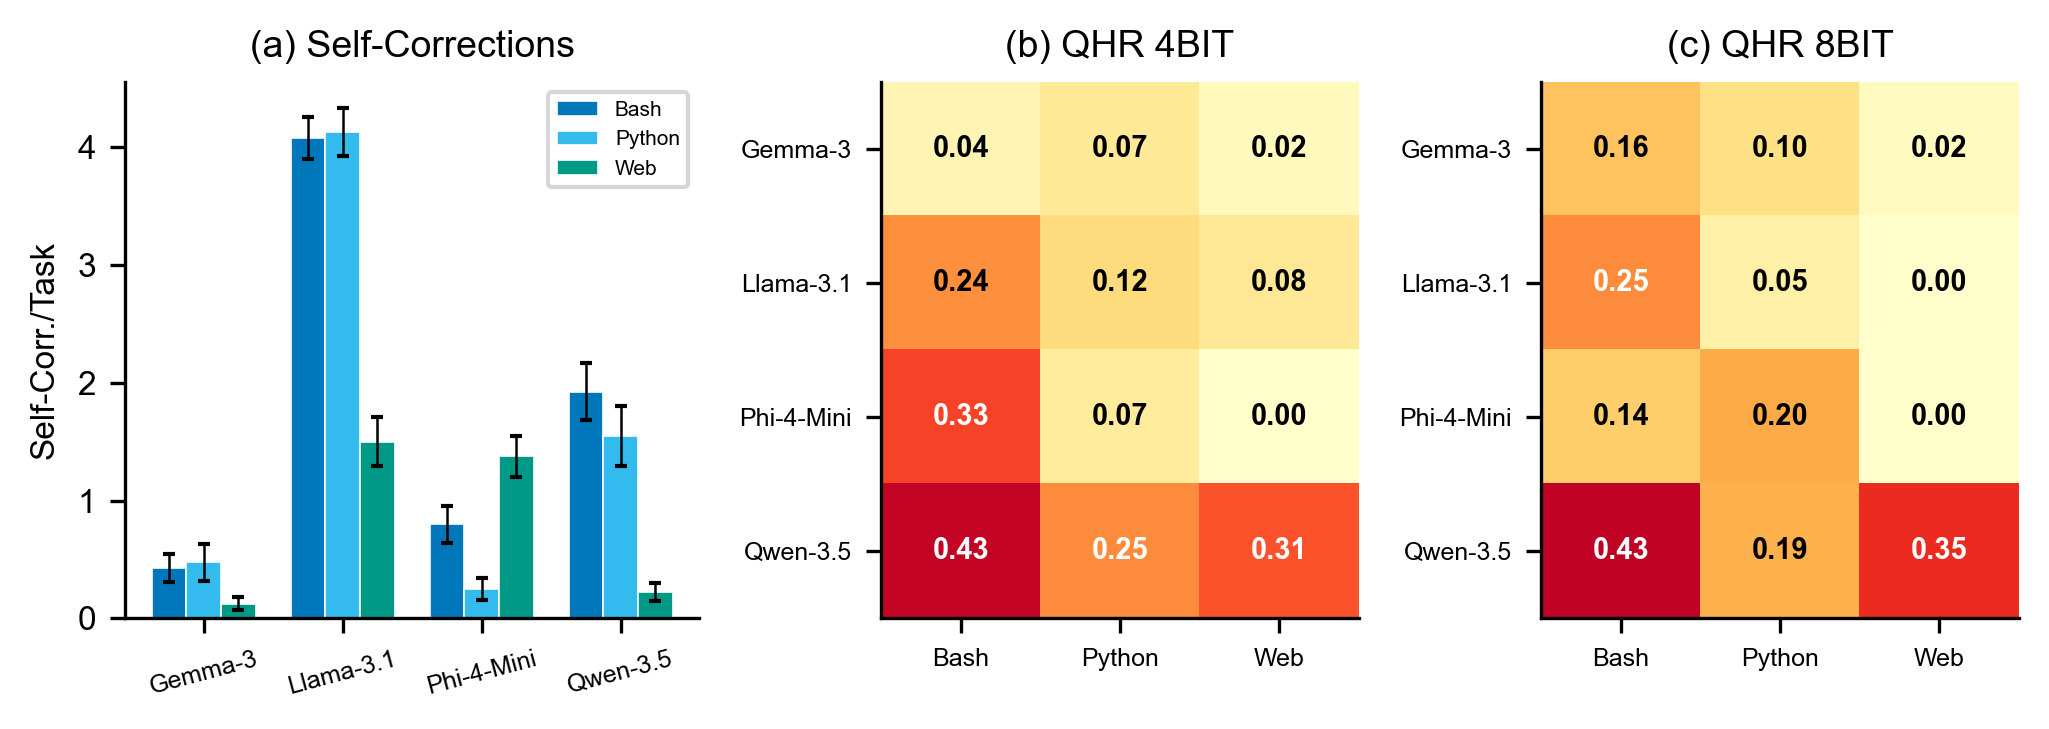
\includegraphics[width=\textwidth]{charts/fig_combined_selfcorr_qhr.png}
  \caption{(a)~Mean self-corrections per task with SEM error bars. More corrections $\neq$ higher success: Llama triggers the most but achieves $<$1\% success. (b,c)~QHR heatmaps for 4-bit and 8-bit. Qwen-3.5's high QHR is architectural, not quantization-dependent.}
  \label{fig:selfcorr_qhr}
\end{figure}

\begin{figure}[t]
  \centering
  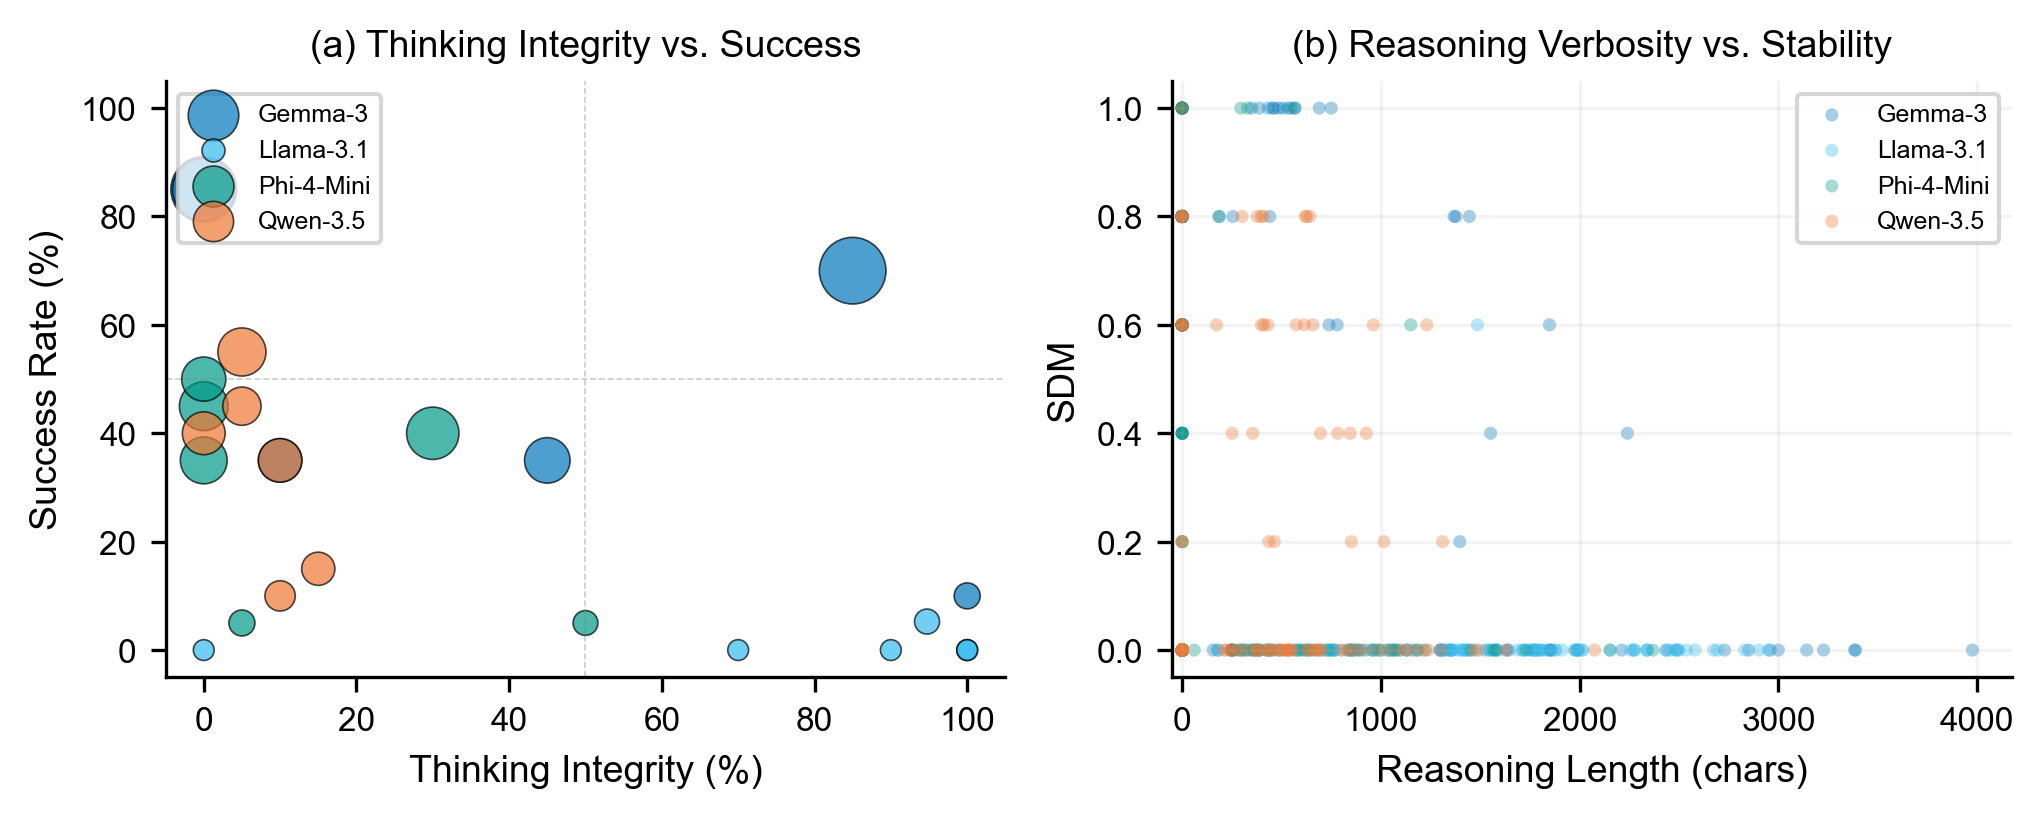
\includegraphics[width=\textwidth]{charts/fig_combined_integrity_reasoning.png}
  \caption{(a)~Thinking integrity vs.\ success rate (bubble $\propto$ SDM). Integrity is necessary but not sufficient: Llama maintains ${\sim}60\%$ integrity at ${\sim}0\%$ success. (b)~Reasoning length vs.\ SDM. Qwen-3.5's verbose reasoning (${\sim}2$--5K chars) consumes generation budget without improving stability. SDM takes discrete values; apparent bands reflect its formulation.}
  \label{fig:integrity_reasoning}
\end{figure}

Figure~\ref{fig:selfcorr_qhr}a reveals a counter-intuitive finding: more self-corrections do not correlate with higher success. Gemma-3 uses fewer corrections but achieves the highest success, as its initial outputs are more reliably correct. Figure~\ref{fig:integrity_reasoning}a shows a positive but non-linear relationship between thinking integrity and success rate, saturating above 80\% integrity. Gemma-3 configurations cluster in the high-integrity, high-success quadrant.

\begin{figure}[t]
  \centering
  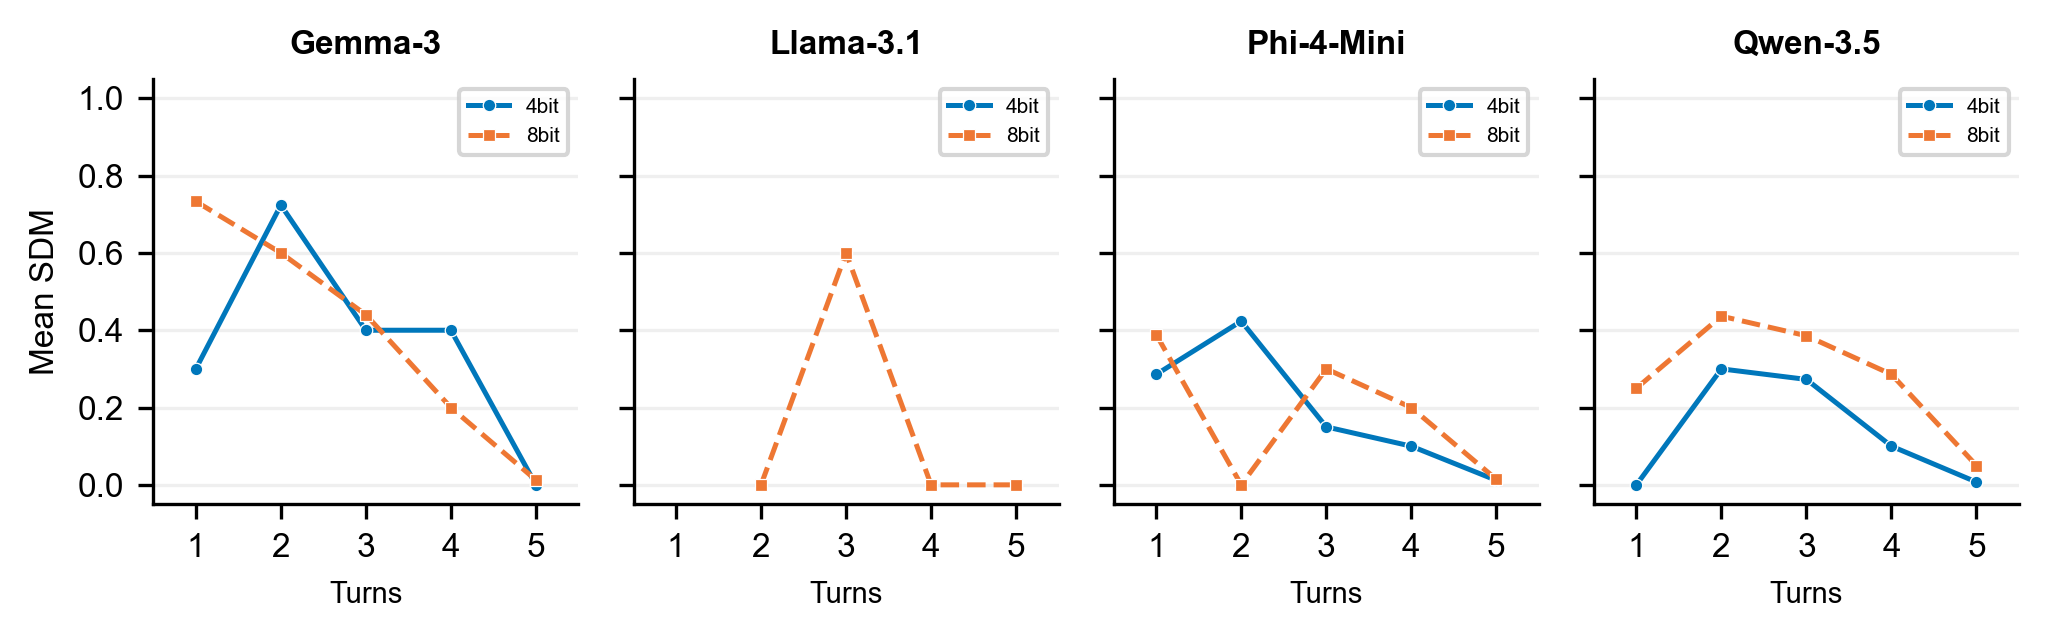
\includegraphics[width=\textwidth]{charts/fig11_sdm_by_turns.png}
  \caption{Stability decay: mean SDM by turn count. Gemma-3 peaks at turns 1--2 then decays; Llama-3.1 shows zero SDM across all turns. 4-bit (solid) vs.\ 8-bit (dashed).}
  \label{fig:sdm_turns}
\end{figure}

Figure~\ref{fig:sdm_turns} directly visualizes stability decay. Gemma-3 achieves SDM $\geq 0.5$ at turns 1--2, dropping sharply thereafter. Llama-3.1's flat zero confirms it never completes tasks regardless of opportunity.

\subsection{Error Taxonomy and Environment Analysis}

\begin{figure}[t]
  \centering
  \begin{subfigure}[b]{0.48\textwidth}
    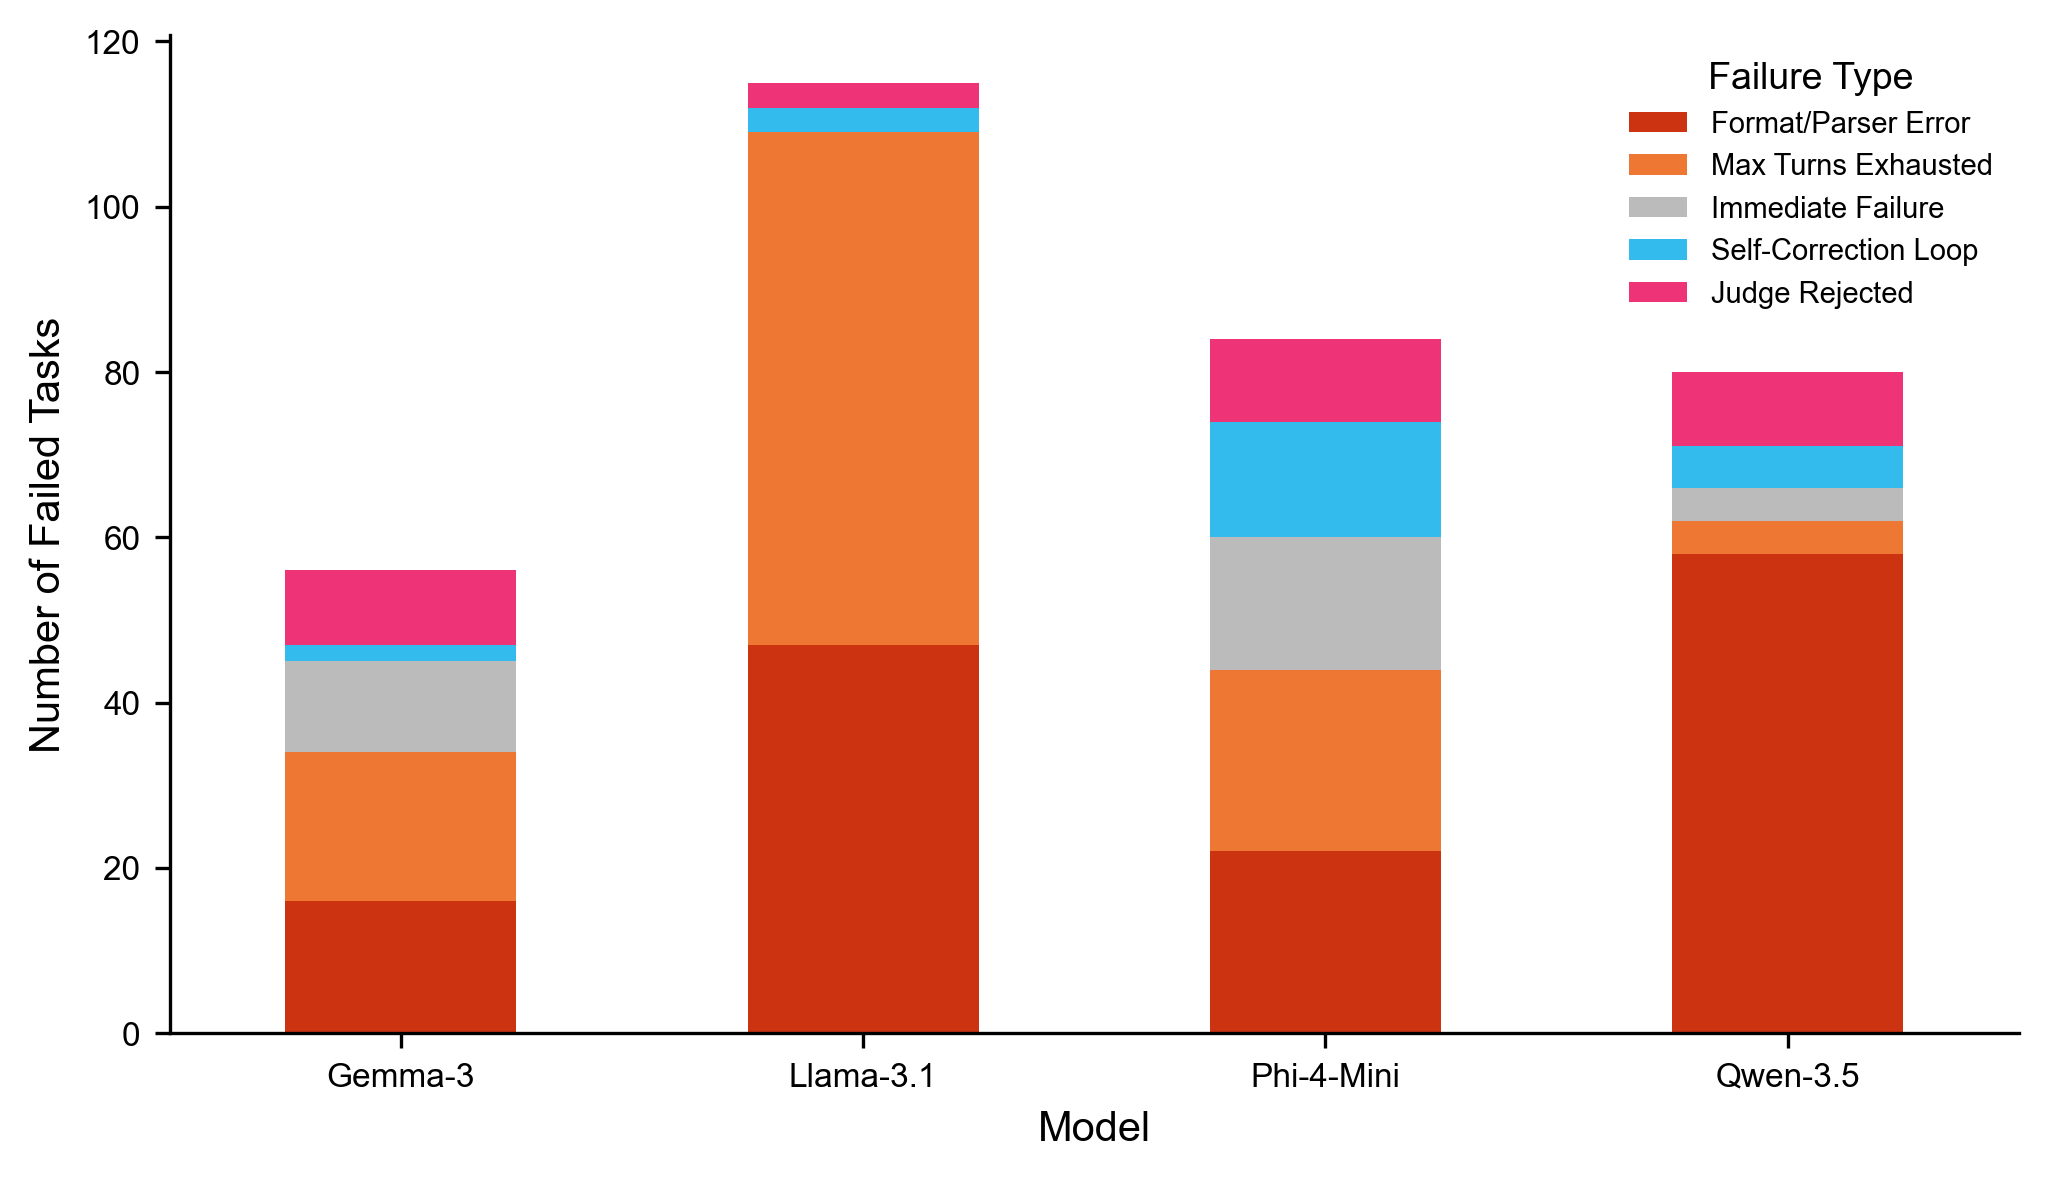
\includegraphics[width=\textwidth]{charts/fig8_error_taxonomy.png}
    \caption{Error taxonomy. Llama: stagnation (53.9\% Max Turns). Qwen: leakage (72.5\% Format Errors).}
    \label{fig:errors}
  \end{subfigure}
  \hfill
  \begin{subfigure}[b]{0.48\textwidth}
    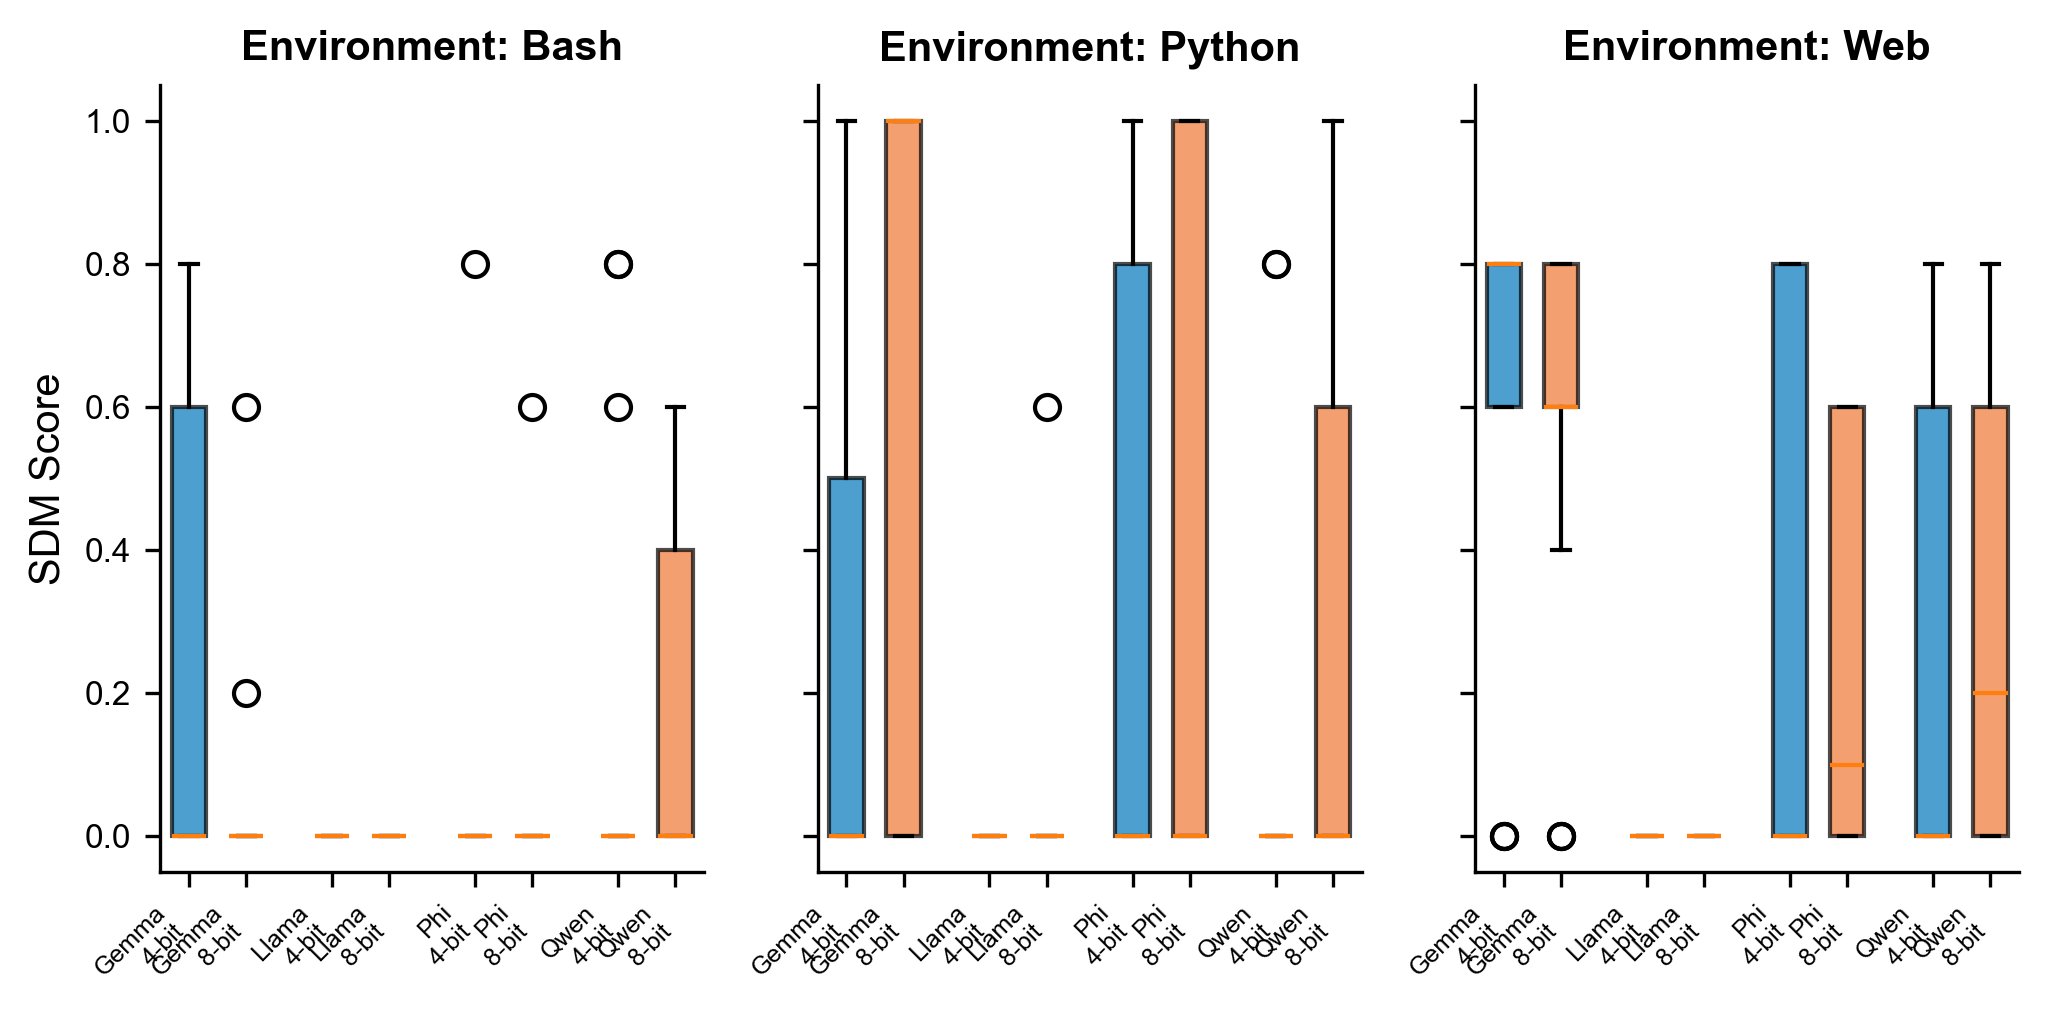
\includegraphics[width=\textwidth]{charts/fig3_sdm_boxplot_by_env.png}
    \caption{SDM by environment. Web is most forgiving; Bash most challenging.}
    \label{fig:env_perf}
  \end{subfigure}
  \caption{Error distribution and environment-level analysis across 335 failed and 476 total tasks.}
  \label{fig:error_env}
\end{figure}

Across 335 failures: Format/Parser Errors dominate (42.7\%), followed by Max Turns Exhausted (31.6\%), Immediate Failures (9.3\%), Judge Rejected (9.3\%), and Self-Correction Loops (7.2\%). Error distributions vary systematically by model (Fig.~\ref{fig:errors}). Web Synthesis is the most forgiving environment ($\overline{\text{SDM}}=0.273$); Bash the most challenging ($\overline{\text{SDM}}=0.082$); Python occupies the middle ($\overline{\text{SDM}}=0.232$) where iterative debugging partially compensates for initial errors (Fig.~\ref{fig:env_perf}). Seven tasks achieved 0\% success across all configurations, all requiring $\geq$4 interdependent steps.

% ============================================================
\section{Discussion}
% ============================================================

\paragraph{Multi-Step Reasoning as a Composite Capability.}
Our qualitative analysis reveals that agentic reasoning is not monolithic but decomposes into four independently degradable sub-capabilities, which we term \textbf{Agentic Sub-Capability Decomposition (ASCD)}: (i)~\emph{plan decomposition}---breaking complex objectives into sequential steps; (ii)~\emph{state tracking}---maintaining awareness of completed vs.\ remaining steps; (iii)~\emph{format adherence}---generating syntactically valid outputs matching the expected schema; (iv)~\emph{completion signaling}---reliably indicating task termination~\cite{wang2024survey,xi2023rise}. Each sub-capability can fail independently: Qwen-3.5 excels at (i) but fails at (iii); Llama-3.1 fails entirely at (ii); Gemma-3 maintains all four consistently; Phi-4-Mini fails at (iv). Table~\ref{tab:arch_failure} maps each model's dominant failure to its architectural root cause and a targeted, deployable mitigation.

\begin{table}[h]
\caption{Architecture--failure--mitigation mapping. Each model's dominant failure archetype is traced to a specific architectural component, yielding targeted interventions deployable without model retraining.}
\label{tab:arch_failure}
\centering
\small
\begin{tabular}{@{}llll@{}}
\toprule
Model & Failed Sub-Capability & Root Cause & Mitigation \\
\midrule
Qwen-3.5 & Format Adherence & Native \texttt{</think>} conflicts with \texttt{<thought>} & Output sanitization \\
Llama-3.1 & State Tracking & Trajectory window discards early context & Explicit state summaries \\
Gemma-3 & Code Generation & 400-token budget truncates long scripts & Dynamic token budgeting \\
Phi-4-Mini & Completion Signaling & No explicit \texttt{[TASK\_COMPLETE]} requirement & Add completion prompt \\
\bottomrule
\end{tabular}
\end{table}

\paragraph{Agentic Competence Hierarchy.}
Based on our data, we propose three tiers (defined by success rate $ > 50\%$, $30$--$50\%$, and $< 5\%$ respectively):
\textbf{Tier 1} (Agentic-Ready): Gemma-3---balanced error profile, effective self-correction, deployable with standard guardrails.
\textbf{Tier 2} (Conditionally Agentic): Phi-4-Mini, Qwen-3.5---dominant single failure mode, deployable with task-specific mitigations.
\textbf{Tier 3} (Not Agentic): Llama-3.1---fundamental state-tracking failure requiring architectural augmentation~\cite{shinn2023reflexion}.

\paragraph{The Quantization Paradox.}
Our environment-dependent finding challenges the assumption that higher precision universally improves performance. In format-constrained environments (Bash), lower precision preserves shorter-range structural attention patterns sufficient for single-command generation. In semantically complex environments (Python), higher precision preserves the long-range syntactic dependencies necessary for complete code generation~\cite{colm2025quantization}. The code truncation archetype directly evidences this: 4-bit Gemma-3 truncates Python code more frequently than 8-bit ($p{=}0.009$), suggesting that 4-bit's reduced weight fidelity specifically degrades the model's ability to track open syntactic constructs (brackets, parentheses, triple-quoted strings) across long generation sequences.

\paragraph{Structural vs.\ Logical Failure.}
Supporting COLM 2025 findings~\cite{colm2025quantization}, we observe that quantization primarily attacks \emph{structural} rather than \emph{logical} reasoning. In our traces, failing models frequently produced coherent reasoning inside \texttt{<thought>} tags while the corresponding action output was syntactically malformed. On the Sieve of Eratosthenes task (py\_7), Gemma-3 8-bit's reasoning trace correctly described the algorithm---``Create a boolean array of size 101, set 0 and 1 to False, iterate from 2 to $\sqrt{100}$''---but the generated code truncated at \texttt{if primes[i}. The model's ``reasoning engine'' is demonstrably more resilient to quantization than its ``formatting engine,'' suggesting that format-level guardrails~\cite{dong2025acbench} may be more impactful than precision upgrades.

\paragraph{Deployment Recommendations.}
Our findings suggest three concrete interventions for deploying quantized SLM agents:
\begin{enumerate}[nosep]
  \item \textbf{Output sanitization} for models exhibiting reasoning leakage: strip content between reasoning tags before parsing action blocks~\cite{schick2023toolformer}.
  \item \textbf{Dynamic token budgeting} for code-generation tasks: increase \texttt{max\_new\_tokens} proportionally to task complexity to prevent truncation.
  \item \textbf{Explicit state summaries} injected into the prompt for models with poor state tracking: provide a structured ``completed steps'' checklist to compensate for attention degradation.
\end{enumerate}

% ============================================================
\section{Limitations}
% ============================================================
\label{sec:limitations}

\begin{enumerate}[nosep,leftmargin=*]
  \item \textbf{Single-run design.} Each configuration was run once ($n{=}20$ tasks) without repeated seeds, a design constraint imposed by the $\sim$24 GPU-hours required across 24 configurations on free-tier Colab (which enforces session timeouts and daily usage limits). We mitigate this in three ways: (a)~exact binomial (Clopper-Pearson) 95\% confidence intervals on success rates (reported in Section~4.1), which quantify sampling uncertainty without requiring repeated runs; (b)~rank-biserial effect sizes alongside all Mann-Whitney $U$ tests, confirming medium-to-large effects ($r{=}0.275$--$0.448$) for significant comparisons; and (c)~the 20-task design provides within-configuration variance across diverse task difficulties, analogous to a stratified evaluation sample. We note that single-run evaluation is common in resource-constrained agent benchmarks (e.g., AgentBench~\cite{liu2023agentbench} reports single-run results for large-scale evaluations). The non-overlapping binomial CIs between Gemma-3 [43.8, 62.6] and Llama-3.1 [0.02, 4.71] confirm that our primary conclusions are robust. However, marginal comparisons (e.g., Qwen Python $p{=}0.078$) should be interpreted cautiously, and multi-seed replication would strengthen effect estimates.
  \item \textbf{Hardware coupling.} All experiments used NVIDIA T4 GPUs via \texttt{bitsandbytes}. Behaviors on Apple Silicon (MLX), Hopper GPUs, or alternative quantization methods (AWQ~\cite{lin2024awq}, GPTQ~\cite{frantar2023gptq}) may differ significantly.
  \item \textbf{LLM-as-a-Judge bias.} Self-evaluation introduces systematic bias; our estimated false-negative rate is $\sim$12\% (6/50 sampled rejections were correct completions).
  \item \textbf{Context window constraint.} $D_{\max}{=}5$ turns limits long-horizon stability observation. Extending to 10--20 turns would enable studying catastrophic degradation patterns.
  \item \textbf{Template sensitivity.} Different SLMs use different chat templates (Gemma's turn-taking, Qwen's \texttt{</think>} tags, Llama's system tokens), which may confound QHR measurements.
  \item \textbf{Trajectory injection asymmetry.} Bash and Python environments use a sliding window of 2 turn-pairs, while Web retains the full trajectory. This design choice may partially explain Web's higher SDM ($0.273$); we did not ablate windowing strategies, and future work should evaluate the effect of window size on agent stability.
  \item \textbf{Benchmark coverage.} Our custom 60-task benchmark was designed to enable controlled, reproducible evaluation within a single Colab session ($\sim$1 hour per configuration). While integration with established benchmarks such as AgentBench~\cite{liu2023agentbench} and WebArena~\cite{zhou2024webarena} would strengthen external validity, these require infrastructure beyond free-tier constraints; our benchmark enables exact reproduction of all reported results on identical hardware.
  \item \textbf{Single-coder qualitative analysis.} Archetype identification was performed by a single researcher; independent replication with inter-rater reliability assessment is needed.
\end{enumerate}

% ============================================================
\section{Broader Impact}
% ============================================================

This work evaluates SLMs as autonomous agents capable of executing system commands and generating code. Several ethical considerations arise:

\textbf{Deployment risks.} Our overall success rate of 29.6\% means that a majority of agent actions fail---including producing syntactically malformed commands that could have unintended side effects in production environments. Deploying such agents without human-in-the-loop oversight, output sandboxing, and rollback mechanisms poses safety risks, particularly in system administration (Bash) contexts where commands modify filesystem state.

\textbf{Quantization trade-offs.} Our finding that lower precision can sometimes outperform higher precision (Section~4.2) cautions against blanket ``more bits = safer'' assumptions in safety-critical deployments. Practitioners must empirically validate quantization effects in their specific deployment environments.

\textbf{Positive impact.} By demonstrating that sub-5B models can achieve meaningful agentic capability on free-tier hardware, this work contributes to democratizing AI agent research beyond well-resourced institutions, enabling researchers with limited compute budgets to develop and evaluate agentic systems locally with full data privacy.

% ============================================================
\section{Conclusion}
% ============================================================

This paper provides the first systematic evaluation of multi-turn recursive stability in quantized SLM agents on resource-constrained hardware. Our key findings challenge simplistic assumptions about quantization:

\begin{itemize}[nosep]
  \item \textbf{Quantization effects are environment-dependent:} 4-bit quantization can be superior in format-constrained tasks but inferior in code-generation tasks, with statistically significant differences ($p < 0.05$).
  \item \textbf{Model size $\neq$ agentic capability:} The largest model (Llama-3.1, 8B) failed catastrophically while smaller models (Gemma-3, Phi-4-Mini, both $\sim$4B) achieved meaningful agentic performance.
  \item \textbf{Format adherence is the primary bottleneck:} 42.7\% of failures stem from parser/format errors rather than logical reasoning failures, suggesting that post-processing and output sanitization may be more impactful than precision upgrades.
\end{itemize}

We release our evaluation harness, all 476 reasoning traces, and the combined dataset to support future research in quantized agentic AI on edge hardware. Future work should prioritize multi-seed replication to narrow confidence intervals, extend $D_{\max}$ to 10--20 turns for long-horizon stability analysis, and validate findings across alternative quantization methods (AWQ, GPTQ) and hardware platforms.

\begin{ack}
We thank the open-source teams behind Qwen, Llama, Gemma, and Phi, the \texttt{bitsandbytes} and HuggingFace communities, and Google Colab for free GPU access. \textbf{Reproducibility:} All experiments used Colab free-tier T4 GPUs, March 3--12, 2026. The harness, 24 trace files, and dataset (476$\times$16) are at the project repository (redacted). \textbf{AI Disclosure:} AI-assisted tools were used for LaTeX formatting, code analysis, and iterative manuscript refinement; all experimental design, data collection, qualitative coding, and scientific interpretation were performed by the author.
\end{ack}

\bibliographystyle{abbrvnat}
\bibliography{references}

\end{document}
